\chapter{Verificación y validación}
\label{CapituloPruebas}
\par En este capitulo se exponen los diferentes ciclos de verificación y validación llevados adelante durante el desarrollo de este proyecto.
\par En primer lugar son presentadas las inspecciones realizadas sobre el sistema durante su desarrollo. Luego, son expuestas una serie de pruebas aplicadas sobre el producto final con el objetivo de asegurar la correcta ejecución y despliegue de resultados. Finalmente, son exhibidas pruebas de campo realizadas a partir de diferentes experimentos de maceración, monitoreados por el sistema, de manera de validar que el mismo se comporte según lo esperado.

\section{Inspecciones del sistema}

Durante el ciclo de vida del proyecto, de forma constante y repetitiva, fueron analizados los requerimientos funcionales y no funcionales, así como las especificaciones formuladas durante el diseño. De esta forma, luego de implementar e integrar funcionalidades en los componentes desarrollados se analizó la documentación de forma de asegurar que se cumpliera con todos los requisitos y requerimientos.

\par Junto al avance del desarrollo de los componentes fueron aplicadas las siguientes pruebas estáticas de forma de comprobar que las funcionalidades cumplieran su objetivo de manera individual e integral:

\begin{itemize}
    \item Pruebas en Componente de Hardware: Recolección de datos de sensores; Inserción en base de datos.
    \item Pruebas de Interfaz Hardware-Software: Verificación de funcionamiento de la \textit{API REST} desarrollada. La \textit{API REST} fue probada utilizando la herramienta \textit{Postman}\footnote{\textit{Postman}, Entorno de desarrollo de \textit{APIs} \url{https://www.getpostman.com/}}. Mediante esta herramienta se proveyeron datos a la \textit{API REST} de la misma forma en que luego serían provistas por la aplicación, así fueron identificados y corregidos distintos fallos.
    \item Pruebas de la aplicación: Verificación de funcionalidades, de manera individual, imprimiendo en el retorno del sistema (\textit{Log}) del entorno de desarrollo \textit{AndroidStudio} diferentes variables de control, verificando así el correcto funcionamiento. En forma adicional, fueron probadas todas las funcionalidades que interactúan de forma integral con el sistema (métodos de interacción con la \textit{API REST}).
\end{itemize}

\par La tabla \ref{tab:TablaChequeoRequerimientos} refleja el cumplimiento de los requerimientos del sistema.
 \begin{table}[H]
     \centering
     \begin{tabularx}{\textwidth}{|X|X|}
     \hline
     \multicolumn{1}{|c|}{Requerimiento} & \multicolumn{1}{|c|}{Verificación}\\
     \hline
     \hline
        \multicolumn{1}{|c|}{RF001}  & El sistema implementa el uso de sensores de temperatura, pH y temperatura ambiente. Mencionados en el capítulo \textit{\textbf{Hardware}}. \\
        \hline
        \multicolumn{1}{|c|}{RF002}  & El sistema implementa el uso de cuatro sensores de temperatura ubicados en distintas posiciones del macerado. El uso de los mismos se menciona en el capítulo \textit{\textbf{Hardware}}. \\
        \hline
        \multicolumn{1}{|c|}{RF003}  & El sistema permite visualizar los datos recolectados por los sensores aun si no se esta llevando a cabo un experimento. Mencionado en el capítulo \textit{\textbf{Software}}. \\
        \hline
        \multicolumn{1}{|c|}{RF004}  & El sistema permite realizar el seguimiento de un experimento de maceración.  Mencionado en el capítulo \textit{\textbf{Software}}.   \\
        \hline
        \multicolumn{1}{|c|}{RF005}  & El sistema permite ingresar todos los datos que caracterizan a una planificación de maceración. Mencionado en el capítulo \textit{\textbf{Software}}.  \\
        \hline
        \multicolumn{1}{|c|}{RF006}  & El sistema permite crear o eliminar una maceración planificada y todos los experimentos relacionados a ella. Mencionado en el capítulo \textit{\textbf{Software}}. \\
        \hline
        \multicolumn{1}{|c|}{RF007}  & El sistema almacena y elimina los datos de los experimentos realizados mediante la interfaz gráfica de la aplicación. Mencionado en el capítulo \textit{\textbf{Software}}. \\
        \hline
        \multicolumn{1}{|c|}{RF008}  & El sistema realiza cálculos de insumos en forma teórica y práctica. En forma adicional, para maceraciones complejas, brinda los cálculos de volumen y temperatura del agua. Mencionado en el capítulo \textit{\textbf{Software}}. \\
        \hline
        \multicolumn{1}{|c|}{RF009}  & El sistema provee información relativa al proceso del experimento de maceración  monitoreado. Mencionado en el capítulo \textit{\textbf{Software}}.  \\
        \hline
        \multicolumn{1}{|c|}{RF010}  & El sistema provee gráficas relativas a los datos recolectados en cada experimento de maceración, además provee otras a partir de resultados obtenidos del conjunto de experimentos. Mencionado en el capítulo \textit{\textbf{Software}}. \\
        \hline
        \multicolumn{1}{|c|}{RF011}  & Luego de 3 experimentos de maceraciones concretados para una misma maceración, el sistema comienza a optimizar los insumos. Mencionado en el capítulo \textit{\textbf{Software}}. \\
        \hline
        \end{tabularx}
        \caption{Tabla de chequeo de requerimientos}
        \label{tab:TablaChequeoRequerimientos}
        \end{table}
        
         \begin{table}[H]
        \centering
        \begin{tabularx}{\textwidth}{|X|X|}
        \hline
        \multicolumn{1}{|c|}{Requerimiento} & \multicolumn{1}{|c|}{Verificación}\\
        \hline
        \multicolumn{1}{|c|}{RF012}  & Durante el monitoreo de un experimento, el sistema permite configurar que sensores intervienen en el cálculo de medidas de representatividad, además de cambiar la forma en que se calcula esta. Mencionado en el capítulo \textit{\textbf{Software}}. \\
        \hline
        \multicolumn{1}{|c|}{RNF001}  & La aplicación utiliza un diseño intuitivo y dinámico, la información es presentada en forma clara (sin ambigüedades). Mencionado en el capítulo \textit{\textbf{Software}}. \\
        \hline
        \multicolumn{1}{|c|}{RNF002}  & Al momento de elegir los diferentes componentes se tuvo en cuenta esta limitación, optando así por los mas económicos.\\
        \hline
        \multicolumn{1}{|c|}{RNF003}  & La plataforma elegida para la aplicación, \textit{Android},  se basó en este requerimiento. Mencionado en el capítulo \textit{\textbf{Hardware}}. \\
        \hline
        \multicolumn{1}{|c|}{RNF004}  & El sistema produce resultados aceptables para recolectar un conjunto de valores, luego el lapso consumido para el envío de los datos a la aplicación es despreciable. \\
        \hline
     \end{tabularx}
     \caption{Tabla de chequeo de requerimientos}
 \end{table}

\section{Pruebas de ejecución y despliegue de resultados}

\par En esta sección se describen las validaciones realizadas a las funcionalidades del sistema mediante distintos tipos de pruebas dinámicas.

\subsection{Funcionamiento de la aplicación}
El correcto funcionamiento de la aplicación se lleva a cabo mediante casos de prueba de tipo ``Entrega''. Según \cite{Som05} "\ldots Las pruebas de entrega, “pruebas funcionales” o “pruebas de caja negra”, son aquellas en las que sólo interesan las funcionalidades del sistema y no su implementación. En otras palabras, se valida que el sistema satisfaga sus requerimientos \ldots".
Las fichas de Casos de Prueba se encuentran ubicadas en el Anexo \ref{CasosPrueba}. Los casos de pruebas son ejecutados por el único usuario del sistema, el fabricante de cerveza Artesanal. Al final de cada ficha bajo el título de ``Evidencias'', se ubica un hipervínculo a un vídeo, donde podrá observarse la ejecución de la prueba.

\subsection{Cálculo de insumos}
\par Se procedió a realizar la validación de los cálculos de insumos implementados mediante el uso de recetas provistas por los directores. Es de resaltar que en el cálculo de insumos utilizado para las validaciones se lleva adelante un procedimiento en el cual no es tenido en cuenta el extracto potencial máximo de cada malta, asumiendo así este potencial como del 100\%. Siendo que los extractos potenciales se encuentran en el intervalo de 70\% a 85\%, los valores aquí calculados serán entre un 15\% a un 30\% mayores según el caso. Tomando en cuenta lo antes mencionado, se consideran como válidos los cálculos que se encuentren dentro de estos intervalos.

%; Parte de un valor de relación agua-grano (aproximación al objetivo de densidad), busca un resultado de mosto final prefijado y para encontrarlo utiliza valores incrementales de cantidad total de insumo hasta que el volumen de salida bajo esa relación satisfaga el objetivo; luego, sobre este total de insumo aplica los porcentajes de la receta para establecer cuanto debe utilizar de cada grano. Por tanto, los valores obtenidos mediante los cálculos aquí implementados variaran respecto de los provistos debido a la injerencia de la ponderación del extracto potencial máximo de cada grano

En la tabla \ref{tab:TablaRecetaExperimentos}, se presentan las recetas y la comparativa de los valores de insumos allí presentes con los obtenidos por la aplicación.
\begin{table}[H]
    \centering
    \begin{tabularx}{\textwidth}{|X|X|X|X|X|X|X|}
    \hline
        Nombre Receta & Granos & Porcentaje & Volumen & Densidad Objetivo & Insumo Receta & Insumo Calculado \\
        \hline
        \hline
        \multirow{2}{2cm}{English Pale Ale} & Pilsen &\multicolumn{1}{c|}{86\%}  &\multirow{2}{2cm}{48.6 litros}  &\multirow{2}{2cm}{1.090} & \multicolumn{1}{c|}{14.04 Kg.} & \multicolumn{1}{c|}{17.34 Kg.}\\
         & Munich & \multicolumn{1}{c|}{14\%} & & &\multicolumn{1}{c|}{2.35 Kg.} &\multicolumn{1}{c|}{2.86 Kg.} \\
        \hline
        \multirow{3}{2cm}{American Blonde Ale} & Pilsen &\multicolumn{1}{c|}{86\%}  &\multirow{3}{2cm}{38.7 litros}  &\multirow{3}{2cm}{1.080} & \multicolumn{1}{c|}{9.47 Kg.} & \multicolumn{1}{c|}{12.28 Kg.}\\
         & Malted Wheat & \multicolumn{1}{c|}{7\%} & & &\multicolumn{1}{c|}{0.87 Kg.} &\multicolumn{1}{c|}{0.96 Kg.}\\ 
         & Carapils & \multicolumn{1}{c|}{7\%} & & & \multicolumn{1}{c|}{0.87 Kg.} &\multicolumn{1}{c|}{1.12 Kg.} \\
        \hline
        \multirow{5}{2cm}{New England IPA} & Pilsen &\multicolumn{1}{c|}{80\%}  &\multirow{5}{2cm}{43.7 litros}  &\multirow{5}{2cm}{1.090} & \multicolumn{1}{c|}{9.6 Kg.} & \multicolumn{1}{c|}{14.51 Kg.}\\
         & Oats & \multicolumn{1}{c|}{10\%} & & &\multicolumn{1}{c|}{1.26 Kg.} &\multicolumn{1}{c|}{1.84 Kg.} \\
        & Carapils & \multicolumn{1}{c|}{4\%} & & &\multicolumn{1}{c|}{0.61 Kg.} &\multicolumn{1}{c|}{0.98 Kg.} \\
        & Wheat & \multicolumn{1}{c|}{3\%} & & &\multicolumn{1}{c|}{0.5 Kg.} &\multicolumn{1}{c|}{0.7 Kg.} \\
        & Corn Sugar & \multicolumn{1}{c|}{3\%} & & &\multicolumn{1}{c|}{0.6 Kg.} &\multicolumn{1}{c|}{0.6 Kg.} \\
        \hline
        \multirow{4}{2cm}{Session IPA} & Pilsen &\multicolumn{1}{c|}{62\%}  &\multirow{4}{2cm}{40.5 litros}  &\multirow{4}{2cm}{1.070} & \multicolumn{1}{c|}{7.69 Kg.} & \multicolumn{1}{c|}{8.11 Kg.}\\
         & Cara Munich & \multicolumn{1}{c|}{23.5\%} & & &\multicolumn{1}{c|}{2.9 Kg.} &\multicolumn{1}{c|}{3.47 Kg.} \\
        & Crystal Munich & \multicolumn{1}{c|}{5.5\%} & & &\multicolumn{1}{c|}{0.73 Kg.} &\multicolumn{1}{c|}{0.83 Kg.} \\
        & Carapils & \multicolumn{1}{c|}{9\%} & & &\multicolumn{1}{c|}{1.11 Kg.} &\multicolumn{1}{c|}{1.32 Kg.} \\
        \hline
        \multirow{8}{2cm}{Hopfen - Weizen} & Pilsen &\multicolumn{1}{c|}{44.44\%}  &\multirow{8}{2cm}{44.15 litros}  &\multirow{8}{2cm}{1.070} & \multicolumn{1}{c|}{5.99 Kg.} & \multicolumn{1}{c|}{6.33 Kg.}\\
         & Malted Wheat & \multicolumn{1}{c|}{33.33\%} & & &\multicolumn{1}{c|}{4.5 Kg.} &\multicolumn{1}{c|}{4.58 Kg.} \\
         & Carapils & \multicolumn{1}{c|}{7.4\%} & & &\multicolumn{1}{c|}{0.99 Kg.} &\multicolumn{1}{c|}{1.19 Kg.} \\
         & Caramel Wheat & \multicolumn{1}{c|}{3.7\%} & & &\multicolumn{1}{c|}{0.49 Kg.} &\multicolumn{1}{c|}{0.61 Kg.} \\
         & Biscuit & \multicolumn{1}{c|}{3.7\%} & & &\multicolumn{1}{c|}{0.49 Kg.} &\multicolumn{1}{c|}{0.54 Kg.} \\
         & Ruby & \multicolumn{1}{c|}{3\%} & & &\multicolumn{1}{c|}{0.4 Kg.} &\multicolumn{1}{c|}{0.44 Kg.} \\
         & Munich Best Malz & \multicolumn{1}{c|}{2.2\%} & & &\multicolumn{1}{c|}{0.297 Kg.} &\multicolumn{1}{c|}{0.32 Kg.} \\
         & Chocolate & \multicolumn{1}{c|}{1.5\%} & & &\multicolumn{1}{c|}{0.2 Kg.} &\multicolumn{1}{c|}{0.24 Kg.} \\
        \hline
    \end{tabularx}
    \caption{Recetas empleadas para experimentos}
    \label{tab:TablaRecetaExperimentos}
\end{table}
\par Siendo que los valores presentados en la tabla \ref{tab:TablaRecetaExperimentos} satisfacen los objetivos antes presentados, se asume como exitosa esta prueba.

\subsection{Cálculo de rendimiento}
Para validar la fórmula de rendimiento, se ingresaron al cálculo de rendimiento valores de densidad objetivo, volumen y cantidad de insumos utilizadas y proporcionados por el cálculo de insumos. Se valida el correcto funcionamiento si la ecuación expresa el mismo rendimiento que el utilizado para el cálculo de insumos.

\begin{table}[H]
    \centering
    \begin{tabularx}{\textwidth}{|X|X|X|X|X|X|}
        \hline
        Densidad & Volumen & KgTotal de Insumos & KgTotal de extracto & Rendimiento utilizado & Rendimiento Calculado \\
        \hline
        \hline
        1.070 & 1.1 litros & 0.366 & 0.288 & 0.70 & 0.7038\\ \hline
        1.070 & 40.55 litros & 13.73 & 10.98 & 0.70 & 0.7054 \\ \hline
        1.090 & 43.7 litros & 18.62 & 14.98 & 0.70 & 0.6976 \\ \hline
    \end{tabularx}
    \caption{Tabla de validación del cálculo de rendimiento  }
    \label{tab:rendimiento}
\end{table}

\par Como puede observarse en la Tabla \ref{tab:rendimiento} el error de aproximación es menor al 0,5\% lo cual considera a los valores obtenidos como aceptables. La desviación se debe a los redondeos utilizados en cada cálculo. 

\subsection{Pruebas de velocidad de medición}
\par
Para la realización de las pruebas de velocidad se llevó a cabo un experimento con las siguientes variables: Duración de 10 minutos, e intervalos de medición de 15 segundos y 120 segundos para las mediciones de temperatura y pH respectivamente.
\par 
En primer lugar, en la figura \ref{fig:pruebasdeInsercion} se presenta una captura tomada de la herramienta \textit{phpmyadmin}\footnote{phpMyAdmin es una herramienta escrita en \textit{PHP} para manejar la administración de \textit{MySQL} a través de páginas web, \url{https://www.phpmyadmin.net/}}. En la figura \ref{fig:pruebasdeInsercionFechayHora} se presenta un acercamiento (zoom) de la columna ``fechayhora'' en la cual  pueden observarse los tiempos en los cuales las inserciones fueron realizadas, siendo que el intervalo de medición de temperatura (el mínimo entre ambos intervalos) fue definido en 15 segundos, las diferencias entre una medición y la siguiente toman valores que van entre los 15 y los 22 segundos. En forma consecuente, se establece que un intervalo de medición de temperatura mínimo debe ser de un valor no inferior a los 22 segundos, de esta forma se asegura un intervalo de duración constante entre mediciones.
\begin{figure}[H]
    \centering
    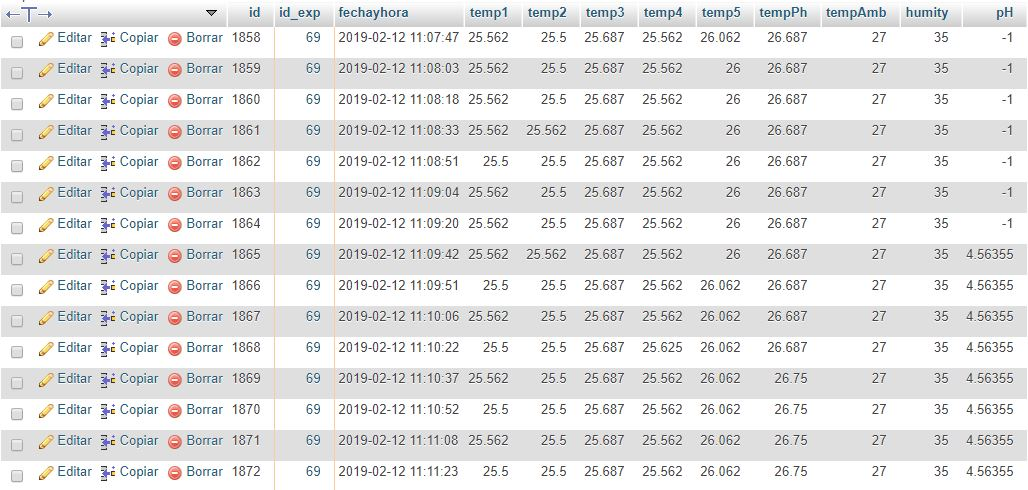
\includegraphics[scale=0.5]{Pruebas/Inserciones.jpg}
    \caption{Captura de mediciones realizadas para la prueba de velocidad}
    \label{fig:pruebasdeInsercion}
\end{figure}
\begin{figure}[H]
    \centering
    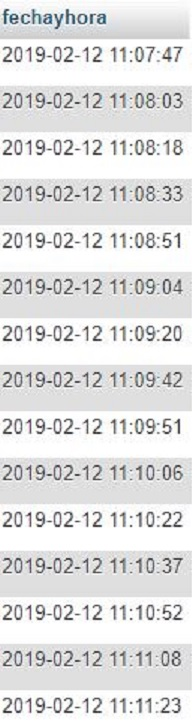
\includegraphics[scale=0.5]{Pruebas/InsercionesZOOM.jpg}
    \caption{Acercamiento de ``fechayhora'' de la tabla de mediciones de pruebas de velocidad}
    \label{fig:pruebasdeInsercionFechayHora}
\end{figure}
\par
Luego, mediante la herramienta \textit{Postman}, fueron realizados tres experimentos. Estos consisten en realizar la consulta de obtención de mediciones a la API REST. En la figura \ref{fig:pruebasdeConsulta} se presentan los resultados, donde puede evidenciarse una demora con duraciones entre 13 ms y 100 ms para obtener la respuesta. A a partir de este valor, se asume a la obtención de datos de la \textit{API REST} como excelente para su propósito.
\begin{figure}[h]
    \centering
    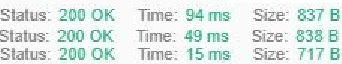
\includegraphics[scale=1]{Pruebas/postman3en1b.jpg}
    \caption{Captura de consulta de mediciones para la prueba de velocidad}
    \label{fig:pruebasdeConsulta}
\end{figure}

\par
Concretadas estas pruebas con un valor de 22 segundos como mínimo para intervalo de medición de temperatura. Se asume satisfactorios los resultados, cumpliendo de esta manera el requerimiento no funcional que motivó la misma.


\section{Pruebas de campo}
\par En esta sección se exponen un conjunto de pruebas experimentales realizadas con el fin de demostrar que los resultados obtenidos por el sistema en el análisis y optimización de insumos cumplen los requerimientos. 

    \subsection{Metodología de pruebas}
        \par Con la finalidad de ejecutar las pruebas se utilizó como macerador un termo\footnote{Termo, adaptación doméstica de un frasco de Dewar} con capacidad volumétrica de 2 litros. Al mismo se le realizaron orificios pasantes de forma de incorporar en su interior los cuatro sensores de temperatura sumergibles, (Figura \ref{fig:ConstrucMacerador}).
        
        \par Los sensores introducidos fueron fijados por medio de pegamento de base siliconada en diferentes posiciones (Figura \ref{fig:ConstrucMacerador}). Con la finalidad de disminuir la pérdida de calor producida por las perforaciones realizadas para introducir estos sensores, se procedió a aplicar sellador siliconado  en los orificios.
        
        \par El termo utilizado cuenta con pico vertedor. El mismo facilita la extracción de muestras sin la necesidad de exponer toda la templa a la temperatura ambiente que produciría la disminución de temperatura y, por tanto, la alteración del experimento.
        
        \par Durante la construcción del macerador, se identificó que el mismo perdía temperatura a un ritmo mayor al aceptable. Por tanto, se procedió a colocar el macerador dentro de un bolso térmico de manera de aumentar el aislamiento. (Figura \ref{fig:ConstrucAislamTerm}).
        
        \par Las mediciones de pH se realizaron a partir de una muestra alojada en un recipiente de aluminio refrigerado (Figura \ref{fig:MedicPH}) para disminuir la temperatura de la solución a la temperatura de calibración (ver Tabla \ref{tablePhvsTemp}). De forma adicional, dentro del recipiente se aloja un sensor de temperatura con el fin de indicar la temperatura de la templa al momento de la medición de pH.
        
        \par Para la realización de los experimentos se optó por utilizar intervalos de medición de 1 minuto para la medición de temperatura y 10 minutos para la obtención de la medida de pH. Si bien el sistema soporta mayor frecuencia de medición de pH, la limitante del volumen del recipiente empleado no permite obtener una cantidad de templa de la cual se puedan extraer demasiadas muestras sin que el total de estas extracciones afecte al resultado final. La cantidad de pruebas se definieron acorde a la realización de diez experimentos por cada tipo de maceración planteada. Es a partir de tres experimentos, que el sistema comienza a realizar ajustes sobre el cálculo de insumos. Luego, con 10 experimentos es posible observar el ajuste de este valor.
        
        \par La malta utilizada para todos los experimentos proviene del mismo lote, y es resguardada en las mismas condiciones. De esta manera puede asegurarse que cualquier cambio de rendimiento obtenido se debe únicamente a la cantidad de insumo utilizado. Definiendo así, las mismas condiciones para todos los experimentos.
        
        En el Anexo \ref{AnexoFotografias} se ubican una serie de imágenes relacionadas a la construcción del sistema y a los procedimientos involucrados en el proceso de maceración.
    \subsection{Recetas y tipos de maceración utilizadas}
        \par Para llevar a cabo los experimentos se planificaron las siguientes maceraciones:
            \subsubsection{Pilsen Lager - Simple} 
                \begin{itemize}
                    \item Tipo de Maceración: Simple
                    \item Volumen: 2 litros
                    \item Densidad específica deseada: 1.070
                    \item Granos:
                        \begin{itemize}
                            \item Nombre: Pilsener \\
                                Porcentaje de utilización: 100\% \\
                                Extracto Potencial: 80\%
                        \end{itemize}
                    \item Intervalos:
                        \begin{itemize}
                            \item Duración: 60 minutos \\
                             Temperatura objetivo: 65°C \\
                             Desvío de temperatura tolerado: ±3°C \\
                             pH: 5.4 \\
                             Desvío de pH tolerado: ±0.2 \\
                        \end{itemize}
                \end{itemize}
                
                \subsubsection{Pilsen Lager - Escalonada} 
                \begin{itemize}
                    \item Tipo de Maceración: Escalonada
                    \item Volumen: 2 litros
                    \item Densidad específica deseada: 1.070
                    \item Granos:
                        \begin{itemize}
                            \item Nombre: Pilsener \\
                                Porcentaje de utilización: 100\% \\
                                Extracto Potencial: 80\%
                        \end{itemize}
                    \item Intervalos:
                        \begin{itemize}
                            \item Duración: 20 minutos \\
                             Temperatura objetivo: 45°C \\
                             Desvío de temperatura tolerado: ±3°C \\
                             pH: 5.4 \\
                             Desvío de pH tolerado: ±0.2 \\
                             \item Duración: 20 minutos \\
                             Temperatura objetivo: 55°C \\
                             Desvío de temperatura tolerado: ±3°C \\
                             pH: 5.4 \\
                             Desvío de pH tolerado: ±0.2 \\
                             \item Duración: 20 minutos \\
                             Temperatura objetivo: 65°C \\
                             Desvío de temperatura tolerado: ±3°C \\
                             pH: 5.4 \\
                             Desvío de pH tolerado: ±0.2 \\
                        \end{itemize}
                \end{itemize}
    \subsection{Valores calculados para cada receta}
    \par A continuación se visualizan los valores calculados por la aplicación para conocer la cantidad de insumos necesaria para realizar la maceración según la planificación correspondiente.
        \subsubsection{Pilsen Lager - Simple}
    
    \begin{minipage}{0.95\textwidth}    
    
        \centering
        \begin{tabularx}{\textwidth}{|X|X|X|X|X|}
             \hline
             \multicolumn{1}{|c|}{Experimentos} & \multirow{1}{2cm}{Rendimiento Utilizado} &\multirow{1}{2cm}{Insumos Utilizados}  & \multirow{1}{2cm}{Rendimiento Obtenido} &\multirow{1}{2cm}{Insumos Ajustados}\\
             & & & &\\
             \hline
             \hline
             \multicolumn{1}{|c|}{1} & \multicolumn{1}{c|}{70\%} & \multicolumn{1}{c|}{0.36 Kg.} &\multicolumn{1}{c|}{60.13\%} &\multicolumn{1}{c|}{-} \\
             \hline
             \multicolumn{1}{|c|}{2} & \multicolumn{1}{c|}{70\%}  & \multicolumn{1}{c|}{0.36 Kg.} &\multicolumn{1}{c|}{61.16\%} &\multicolumn{1}{c|}{-} \\
             \hline
             \multicolumn{1}{|c|}{3} & \multicolumn{1}{c|}{70\%} & \multicolumn{1}{c|}{0.36 Kg.} &\multicolumn{1}{c|}{62.54\%} &\multicolumn{1}{c|}{0.37356 Kg.} \\
             \hline
             \multicolumn{1}{|c|}{4} & \multicolumn{1}{c|}{62.54\%}  & \multicolumn{1}{c|}{0.4 Kg.} &\multicolumn{1}{c|}{63.75\%} &\multicolumn{1}{c|}{0.37777 Kg.} \\
             \hline
             \multicolumn{1}{|c|}{5} & \multicolumn{1}{c|}{63.75\%}  & \multicolumn{1}{c|}{0.37777 Kg.} &\multicolumn{1}{c|}{64.89\%} &\multicolumn{1}{c|}{0.38221 Kg.} \\
             \hline
             \multicolumn{1}{|c|}{6} & \multicolumn{1}{c|}{64.89\%}  & \multicolumn{1}{c|}{0.38221 Kg.} &\multicolumn{1}{c|}{66.17\%} &\multicolumn{1}{c|}{0.39111 Kg.} \\
             \hline
             \multicolumn{1}{|c|}{7} & \multicolumn{1}{c|}{66.17\%}  & \multicolumn{1}{c|}{0.39111 Kg.} &\multicolumn{1}{c|}{66.78\%} &\multicolumn{1}{c|}{0.37673 Kg.} \\
             \hline
             \multicolumn{1}{|c|}{8} & \multicolumn{1}{c|}{66.78\%}  & \multicolumn{1}{c|}{0.37673 Kg.} &\multicolumn{1}{c|}{66.99\%} &\multicolumn{1}{c|}{0.36486 Kg.} \\
             \hline
             \multicolumn{1}{|c|}{9} & \multicolumn{1}{c|}{66.99\%}  & \multicolumn{1}{c|}{0.36486 Kg.} &\multicolumn{1}{c|}{67.14\%} &\multicolumn{1}{c|}{0.36401 Kg.} \\
             \hline
             \multicolumn{1}{|c|}{10} & \multicolumn{1}{c|}{67.14\%} & \multicolumn{1}{c|}{0.36401 Kg.} &\multicolumn{1}{c|}{67.48\%} &\multicolumn{1}{c|}{0.37286 Kg.} \\
             \hline
        \end{tabularx}
        \captionof{table}{Tabla de resultados Pilsen Lager Simple}
        \label{tab:ResultadosPilsenSimple}
    \end{minipage}
    
 \subsubsection{Pilsen Lager - Escalonada}
    
    \begin{minipage}{0.95\textwidth}    
    
        \centering
        \begin{tabularx}{\textwidth}{|X|X|X|X|X|}
             \hline
             \multicolumn{1}{|c|}{Experimentos} & \multirow{1}{2cm}{Rendimiento Utilizado} &\multirow{1}{2cm}{Insumos Utilizados}  & \multirow{1}{2cm}{Rendimiento Obtenido} &\multirow{1}{2cm}{Insumos Ajustados}\\
             & & & &\\
             \hline
             \hline
             \multicolumn{1}{|c|}{1} & \multicolumn{1}{c|}{70\%} & \multicolumn{1}{c|}{0.36 Kg.} &\multicolumn{1}{c|}{51.92\%} &\multicolumn{1}{c|}{-} \\
             \hline
             \multicolumn{1}{|c|}{2} & \multicolumn{1}{c|}{70\%}  & \multicolumn{1}{c|}{0.36 Kg.} &\multicolumn{1}{c|}{62.2\%} &\multicolumn{1}{c|}{-} \\
             \hline
             \multicolumn{1}{|c|}{3} & \multicolumn{1}{c|}{70\%} & \multicolumn{1}{c|}{0.36 Kg.} &\multicolumn{1}{c|}{65.3\%} &\multicolumn{1}{c|}{0.37356 Kg.} \\
             \hline
             \multicolumn{1}{|c|}{4} & \multicolumn{1}{c|}{62.54\%}  & \multicolumn{1}{c|}{0.37356 Kg.} &\multicolumn{1}{c|}{64.27\%} &\multicolumn{1}{c|}{0.36529 Kg.} \\
             \hline
             \multicolumn{1}{|c|}{5} & \multicolumn{1}{c|}{62.97\%}  & \multicolumn{1}{c|}{0.36529 Kg.} &\multicolumn{1}{c|}{65.3\%} &\multicolumn{1}{c|}{0.36828 Kg.} \\
             \hline
             \multicolumn{1}{|c|}{6} & \multicolumn{1}{c|}{63.44\%}  & \multicolumn{1}{c|}{0.36828 Kg.} &\multicolumn{1}{c|}{74.66\%} &\multicolumn{1}{c|}{0.40727 Kg.} \\
             \hline
             \multicolumn{1}{|c|}{7} & \multicolumn{1}{c|}{65.31\%}  & \multicolumn{1}{c|}{0.40727 Kg.} &\multicolumn{1}{c|}{70.49\%} &\multicolumn{1}{c|}{0.38094 Kg.} \\
             \hline
             \multicolumn{1}{|c|}{8} & \multicolumn{1}{c|}{66.05\%}  & \multicolumn{1}{c|}{0.38094 Kg.} &\multicolumn{1}{c|}{72.57\%} &\multicolumn{1}{c|}{0.38705 Kg.} \\
             \hline
             \multicolumn{1}{|c|}{9} & \multicolumn{1}{c|}{66.86\%}  & \multicolumn{1}{c|}{0.38705 Kg.} &\multicolumn{1}{c|}{68.41\%} &\multicolumn{1}{c|}{0.36461 Kg.} \\
             \hline
             \multicolumn{1}{|c|}{10} & \multicolumn{1}{c|}{67.03\%} & \multicolumn{1}{c|}{0.36461 Kg.} &\multicolumn{1}{c|}{70.49\%} &\multicolumn{1}{c|}{0.37341 Kg.} \\
             \hline
        \end{tabularx}
        \captionof{table}{Tabla de resultados Pilsen Lager Escalonada}
        \label{tab:ResultadosPilsenEscalonada}
    \end{minipage}
    
    
    \subsection{Resultados obtenidos}
        \par Para cada receta realizada se muestran las gráficas de promedio de temperatura y pH obtenidas por la aplicación. Las mismas se presentan en el Anexo \ref{GraficasPruebasCampo}.
    
    \subsection{Evaluación}
        \par En la anterior subsección se evidenció que el ajuste de la cantidad de insumos realizada por el sistema produce resultados correctos, esto es, cuando la densidad es menor a la deseada incrementa la cantidad de granos de manera de compensar este sub-rendimiendo, y lo mismo ocurre en caso contrario con un sobre-rendimiento. Esta compensación representa el objetivo de esta funcionalidad, la cual es asistir al productor a partir de una herramienta de optimización de insumos en función de un ajuste utilizando el rendimiento del equipo.
        
        \par Cabe señalar que si bien pueden parecer reducidos los cambios en los valores de insumo, los mismos corresponden a un preparado de un volumen reducido. Estos cambios crecerán en forma proporcional al tamaño del preparado, constituyéndose en valores más significativos conforme a este incremento.
        
        \par Por tanto, puede concluirse que esta funcionalidad del sistema se comporta de la manera esperada, y por tanto, correcta. 
    
    
        
        
%validar el usuario lo acepta, verificar comprobar que lo que haces anda bien, tiene resultados correctos 